% Shared preamble for the CIG-AMF formal-research papers.
% IEEEtran conference class; compiles on Overleaf without modification.
\documentclass[conference]{IEEEtran}
\IEEEoverridecommandlockouts

\usepackage{cite}
\usepackage{amsmath,amssymb,amsfonts}
\usepackage{amsthm}
\usepackage{algorithm}
\usepackage{algorithmic}
\usepackage{graphicx}
\usepackage{textcomp}
\usepackage{xcolor}
\usepackage{booktabs}
\usepackage{url}
\usepackage[hidelinks]{hyperref}

\def\BibTeX{{\rm B\kern-.05em{\sc i\kern-.025em b}\kern-.08em T\kern-.1667em\lower.7ex\hbox{E}\kern-.125emX}}

\newtheorem{theorem}{Theorem}
\newtheorem{lemma}[theorem]{Lemma}
\newtheorem{proposition}[theorem]{Proposition}
\newtheorem{corollary}[theorem]{Corollary}
\theoremstyle{definition}
\newtheorem{definition}[theorem]{Definition}
\newtheorem{remark}[theorem]{Remark}
\newtheorem{example}[theorem]{Example}

% A machine-checked statement carries its Lean declaration name.
\newcommand{\lean}[1]{\textsf{\footnotesize #1}}
\newcommand{\leanbox}[1]{%
  \par\vspace{2pt}\noindent
  {\footnotesize\textsf{Lean: #1}}\par\vspace{2pt}}

% Evidence classes, used consistently and never interchangeably.
\newcommand{\PROVED}{\textsc{proved}}
\newcommand{\CERT}{\textsc{certificate}}
\newcommand{\NUM}{\textsc{numerical}}
\graphicspath{{../_figures/}}


\begin{document}

\title{The Observation Order of a\\Safe Compression Decision}

\author{\IEEEauthorblockN{Vu Phan An Nguyen}
\IEEEauthorblockA{\textit{Rider University} \\
Lawrenceville, NJ, USA}}

\maketitle

\begin{abstract}
A learner that must choose a compression does not have to identify the world it is in; it
only has to separate worlds far enough that no set of them disagreeing on every answer
survives unsplit. We make that quantitative for a measurement class in which the world is
latent and every query is a bounded linear probe. On one explicit family the two costs come
apart by a computable order: the decision is settled at order $h^{-2}$ and identification
needs $h^{-2r}$, with $r$ a design parameter of the family. Three things support the claim.
First, the moment law: for every admissible query of degree $d$ the mixed moments against
the hidden character vanish below order $\lceil n/d\rceil$, and the averaged tail query
attains that order with leading coefficient exactly $r!/r^{r}$---both proved. Second, the
lower bound holds against every adaptive policy on a finite observation alphabet---and, on
the Gaussian model, is reduced to a single per-step Hellinger bound, which we now
\emph{prove}, obtaining $\int\Delta^{2}/\ell\le h^{2r}r^{-2r}C$ with $C$ explicit, leaving
only the continuous-alphabet chain rule between the two---rather
than against a chosen query: we build
the transcript law from the policy and prove the divergence chain rule for it, so the
per-query bound multiplies by the horizon and nothing else. Third, the combinatorial half of
the general law: grouping worlds by equality of their observation coefficients up to order
$s$---an equivalence by construction, not a union-find on an untested relation---every class
has a common safe answer if and only if no obstruction lies inside a class, and against an
obstruction every \emph{randomised} rule leaves unsafe mass at least $1/|H|$. Deciding
without identifying, and signal appearing only at high moments, are both known; what we
claim is the combined law relating safe-decision geometry, a query class, and adaptive
transcripts, with matching orders on one family.
\end{abstract}

\begin{IEEEkeywords}
sequential design, adaptive lower bounds, moment methods, decision regions, formal
verification
\end{IEEEkeywords}

\section{Introduction}
\label{sec:intro}

\subsection{The question}

Identification is sufficient for choosing an action and is usually far more than necessary.
The question is how much more, and whether the gap can be predicted from the structure of
the problem rather than measured after the fact.

Fix $\varepsilon$ and let $\mathcal{A}_{\varepsilon}(F)$ be the set of $\varepsilon$-safe
compressions in world $F$. A set of worlds $H$ is an \emph{obstruction} when
$\bigcap_{F\in H}\mathcal{A}_{\varepsilon}(F)=\varnothing$. Writing $r_{q}(F,G)$ for the
first order at which query $q$'s observation law distinguishes $F$ from $G$, the orders that
should govern the two costs are
\begin{equation}
r_{\rm safe}=\max_{H\in\mathcal{H}}\min_{q}\min_{\substack{F,G\in H\\F\ne G}}r_{q}(F,G),
\qquad
r_{\rm id}=\max_{F\ne G}\min_{q}r_{q}(F,G),
\label{eq:orders}
\end{equation}
with $\mathcal{H}$ the minimal obstructions.

\subsection{What is new, against the nearest sources}

Two ingredients are established and we use them as tools.

\textbf{Deciding without identifying.} Javdani et al.~\cite{javdani2014} formulate decision
making with overlapping decision regions and give near-optimal Bayesian active learning for
it. The idea that a learner may stop short of identification is theirs, not ours.

\textbf{Signal at high moments.} That raising algebraic degree postpones the first
informative moment, and the sample cost with it, is the masking mechanism analysed by Grosso,
Standaert and Prouff~\cite{grosso2014}, with moment expansions of information in the
side-channel setting by Rioul, Cheng and Guilley~\cite{rioul2021}.

Information games with several correct answers, and their decomposition into finitely many
convex regions, are also developed---Degenne and Koolen~\cite{degenne2019}, and more
recently Wang and You~\cite{wangyou2026}. We do not claim that framework. We also do not
claim those works have settled their own algorithmic questions; \cite{wangyou2026} leaves an
exact stopping threshold problem-dependent and labels part of its scaling heuristic.

What is ours is the \emph{combination}, and it is a combination that has content because the
three pieces constrain each other:
\begin{enumerate}
\item[1)] a safe-decision geometry in which the safe sets are computed from a compression
loss, not posited;
\item[2)] a query class for which the order is \emph{proved}, in both directions---vanishing
below $\lceil n/d\rceil$ and attainment at it with an exact constant;
\item[3)] an adaptive transcript bound, so the lower bound is against every policy.
\end{enumerate}
A reader who removes any one of the three gets a statement already in the literature.

\NOTEPAR{The honest framing for the final version: if a masking theorem is found that
already covers the admissible class as stated in Theorem~\ref{thm:vanish}, cite it as a tool
and move the novelty claim entirely to Section~\ref{sec:law}. Do not defend a duplicate.}

\section{The family, and its safe sets}
\label{sec:family}

For $r\ge2$ and $u,v\in\{-1,1\}$ put $X=\{-1,1\}^{r+3}$ and
\begin{equation}
F_{u,v}(z)=3u z_{1}-2z_{2}-2z_{3}+v\prod_{\ell=4}^{r+3}z_{\ell},
\label{eq:family}
\end{equation}
with the uniform product reference and the deployment support
\begin{equation}
K=\bigl\{(t,t,t,1,\dots,1):t=\pm1\bigr\}.
\label{eq:support}
\end{equation}
The single-coordinate responses are $Q_{1}(z_{1})=3uz_{1}$, $Q_{2}=-2z_{2}$, $Q_{3}=-2z_{3}$
and $Q_{j}=0$ for $j\ge4$, and the losses on $K$, computed as half the oscillation of the
retained residual, are
\begin{equation}
L_{K}(\{1\})=4,\quad L_{K}(\{2\})=L_{K}(\{3\})=|3u-2|,\quad L_{K}(\{j\})=|3u-4|
\label{eq:losses}
\end{equation}
for $j\ge4$. Every entry is derived from~\eqref{eq:family} and~\eqref{eq:support}; no loss
table is declared. \CERT{}

Two consequences matter. For $\varepsilon<1$ the safe sets at $u=+1$ and $u=-1$ are
\emph{disjoint}---at $u=-1$ only $\{1\}$ is safe, at $u=+1$ every other singleton is---so a
safe compression rule also decides $u$. And $v$ does not move the safe set at all: the
interaction sign is decision-irrelevant.

\subsection{The observation model, which is where the content is}

A query picks a linear $g$ with $\|g\|_{\infty}\le1$ and returns
\begin{equation}
Y=F_{u,v}(Z)+h\,g(Z)+\xi,\qquad Z\sim\mathrm{Unif}(X),\ \xi\sim N(0,\sigma^{2}).
\label{eq:obs}
\end{equation}
Three conditions are not decoration:
\begin{itemize}
\item $Z$ is \emph{latent} and is never returned;
\item queries may sample on $X$ while the compression is judged on $K$;
\item no query reads $F$ directly, and $g$ may not be amplified by $1/h$.
\end{itemize}

\TODOPAR{If $Z$ were observed, or the class were richer than bounded linear probes, the
lower bound can collapse. If an application forces measurement on $K$ only, the construction
must change; that difference must not be hidden in notation. State this beside the model in
the final version, not in a remark.}

A fact worth isolating: $u$ is \emph{invisible} at order zero. The law of $F$ alone does not
depend on $\mathrm{sign}(u)$, because $z_{1}$ is symmetric; only the probe $h\,g$ breaks that
symmetry. This is why the decision costs $h^{-2}$ rather than $O(1)$, and it is a property of
the construction rather than an assumption. \CERT{}

\section{The order law}
\label{sec:order}

\subsection{Vanishing}

\begin{theorem}[Moment vanishing]
\label{thm:vanish}
Let $\chi$ be the top character on $\{-1,1\}^{n}$ and let $g$ be any polynomial of degree at
most $d$. Then $\mathbb{E}[\chi\,g^{j}]=0$ for every $j$ with $jd<n$, in particular for every
$j<\lceil n/d\rceil$.
\end{theorem}

\leanbox{\lean{moment\_vanishes\_below\_order}, \lean{moment\_vanishes\_below\_s}, with
\lean{chiS\_mul}, \lean{HasDeg\_mul}, \lean{top\_character\_orthogonal}, in
\lean{LeanUnifiedQueryOrderV1}}

The proof is short and is the reason the statement is about \emph{every} admissible query
rather than a chosen one: characters multiply to the character of the symmetric difference,
so degrees add under multiplication, and the only set surviving against the top character is
the full one, which needs $jd\ge n$.

\subsection{Attainment, with the exact constant}

\begin{theorem}[Attainment]
\label{thm:attain}
For the averaged tail query,
$\displaystyle\sum_{z\in\{-1,1\}^{n}}\Bigl(\prod_{i}z_{i}\Bigr)\Bigl(\sum_{i}z_{i}\Bigr)^{k}$
vanishes for $k<n$ and equals $2^{n}\,n!$ for $k=n$. Normalising,
$\mathbb{E}[\chi_{n}g^{n}]=n!/n^{n}\neq0$.
\end{theorem}

\leanbox{\lean{cubeSum\_below\_diag}, \lean{cubeSum\_diag}, \lean{tail\_query\_moment},
\lean{tail\_query\_moment\_ne\_zero} in \lean{LeanPaperBAttainmentV1}}

The proof is a recurrence, not a bijection count: peeling one coordinate and expanding the
binomial gives
\begin{equation}
\mathrm{cubeSum}(n{+}1,k)=\sum_{j}\binom{k}{j}\bigl(1+(-1)^{j+1}\bigr)\,\mathrm{cubeSum}(n,k{-}j),
\label{eq:rec}
\end{equation}
whose parity factor kills every even $j$, so the recursive index always drops strictly and a
single induction gives both lines. Theorems~\ref{thm:vanish} and~\ref{thm:attain} together
turn an $\Omega$ into a $\Theta$.

\subsection{Both scales, on the real family}

On~\eqref{eq:family}, the decision probe $g=z_{1}$ gives
$\mathbb{E}[Y^{2}]=18+\sigma^{2}+6uh+h^{2}$ exactly, so the two values of $u$ sit $12h$
apart; and the order-$(r{+}1)$ moment contrast between $v=\pm1$ under the tail query is
exactly $2(r{+}1)\,r!/r^{r}\,h^{r}$---an identity, not a leading term. \CERT{}

Measuring the squared Hellinger distance of the \emph{actual} observation laws by
deterministic quadrature gives log--log slopes $1.983$ for the decision pair against a
predicted $2$, and $3.959$ and $5.962$ for the identification pair at $r=2,3$ against
predicted $4$ and $6$. \NUM{} Under the wrong probe the identification pair is not merely
higher-order but \emph{exactly} indistinguishable: $H^{2}<10^{-12}$ at every $h$, because
flipping $v$ is a measure-preserving relabelling of the tail coordinates and $z_{1}$ is
independent of them. The order is a property of the query class, not only of the worlds.

\section{Against every adaptive policy}
\label{sec:adaptive}

A per-query bound says nothing about a learner that chooses its next query from what it has
seen. The step that makes the lower bound legitimate is the transcript chain rule, and we
prove it for a transcript law built from the policy rather than assumed to be a product.

\begin{theorem}[Transcript chain rule and horizon bound]
\label{thm:chain}
For a policy $\mathrm{pol}$ mapping histories to queries,
\begin{equation}
\mathrm{KL}_{n+1}(h)=\mathrm{kl}\bigl(P_{\mathrm{pol}(h)},P'_{\mathrm{pol}(h)}\bigr)
+\sum_{o}P_{\mathrm{pol}(h)}(o)\,\mathrm{KL}_{n}(h\!\cdot\!o),
\label{eq:chain}
\end{equation}
and hence $\mathrm{KL}_{N}\le N\sup_{q}\mathrm{kl}(P_{q},P'_{q})$.
\end{theorem}

\leanbox{\lean{klPath\_chain}, \lean{klPath\_le\_horizon}, with \lean{sumPaths\_mass} and
\lean{klPath\_nonneg}, in \lean{LeanPaperBTranscriptKLV1}}

The policy contributes nothing because it is the same map under both worlds. With the
per-query bound of Theorem~\ref{thm:vanish} this gives $N\gtrsim h^{-2r}$ for identification
against every adaptive policy \emph{on a finite observation alphabet}. The observation model
of this paper has Gaussian noise, so Theorem~\ref{thm:chain} does not close the lower bound
on the model we actually use, and we do not claim that it does.

\subsection{What would close it, and what is already proved of that}

The route that does close it runs on the Hellinger \emph{affinity}
$\rho(P,Q)=\int\sqrt{pq}=1-H^{2}(P,Q)$, because a policy that uses the same query kernel
under both worlds contributes a factor of one at every step, so
\begin{equation}
\rho\bigl(\mathbb{P}^{\pi,N}_{+},\mathbb{P}^{\pi,N}_{-}\bigr)\ \ge\
\bigl(1-C_{r}h^{2r}\bigr)^{N},
\label{eq:affinity}
\end{equation}
\emph{provided} the per-step bound $\sup_{g}H^{2}(P^{g}_{+,h},P^{g}_{-,h})\le C_{r}h^{2r}$
holds uniformly over the query class. Two-point testing then gives
$\mathrm{err}_{N}\ge\tfrac14\rho^{2}$.

Everything after that per-step bound is arithmetic, and it is proved: the product in
\eqref{eq:affinity} from a per-step floor, Bernoulli's inequality, and the conclusion that no
budget below $(1-2\sqrt{\delta_{0}})/(C_{r}h^{2r})$ reaches error $\delta_{0}$. The same
statement with $h^{2}$ in place of $h^{2r}$ gives the decision side. So the general adaptive
lower bound is reduced to \emph{one} analytic obligation---a per-step Hellinger bound
uniform over the query class---and to nothing else.

\leanbox{\lean{affinity\_pow\_lower}, \lean{affinity\_bernoulli},
\lean{budget\_lower\_from\_affinity}, \lean{two\_exponents\_from\_affinity} in
\lean{LeanPaperBRatesV1}}

\paragraph{Where this sits, and what it is not.}
The \emph{phenomenon} behind \eqref{eq:affinity} has a clear precedent. The masking and
side-channel literature has studied exactly this mechanism for years: low moments carry no
information, the signal appears only at high order, a coupling or a nonlinearity lowers
the protective order, and changing the noise level changes which regime
dominates~\cite{duc2015}. Duc, Faust and Standaert discuss non-independent leakage
directly. Their treatment has heuristic components and does not contain the adaptive
theorem proved here --- but it does mean that
\[
H^{2}\asymp h^{2r},\qquad N\asymp h^{-2r},
\]
and even the $h^{6}+\eta^{2}h^{4}$ crossover, are \textbf{not} strong enough on their own
to carry a paper. They are recorded here as supporting results.

Likewise, keeping only decision-relevant information is itself an established
idea~\cite{poli2023}. What would have to be new is the \emph{exponent law and its
geometric characterisation}, not the slogan.

The question we therefore keep is:

\begin{quote}
\emph{the order of information needed to find a safe compression can differ from the order
needed to identify the world, already when the safe answer sets overlap and the queries are
chosen adaptively.}
\end{quote}

with the target
\[
N_{\rm safe}(h,\delta)\asymp h^{-2s_{\rm safe}}\log(1/\delta),
\qquad
N_{\rm id}(h,\delta)\asymp h^{-2s_{\rm id}}\log(1/\delta),
\qquad s_{\rm safe}<s_{\rm id},
\]
and three conditions that make it worth more than an easy-target-plus-hard-nuisance
construction: the safe sets must come from the actual \lean{selectedRadius} geometry rather
than an assigned answer table; they must genuinely \emph{overlap}, as in
$\{1,2\},\{2,3\},\{1,3\}$, so that no single nuisance bit can be discarded; and the lower
bound must cover every adaptive policy with a matching upper bound on the same query class.

\NOTEPAR{None of those three is delivered here. What is delivered is the analytic half:
\eqref{eq:affinity} on the linear class with explicit constants, and the
$\log(1/\delta)$ side of the budget below. If the geometry half does not follow, this
material belongs inside the Support paper as a supporting rate, not as a paper of its own.
That is the honest reading and we do not argue against it.}

\paragraph{The remaining obligation, measured.}
Since everything after \eqref{eq:affinity} is proved, the whole adaptive lower bound turns
on one number, and that number can be computed. Both densities are exact finite Gaussian
mixtures, so $\sup_{g}H^{2}$ is a quadrature over the mixtures themselves, with the
supremum attacked by many restarts of a projected ascent over the probe class, with the
canonical construction probe $(z_{4}+z_{5}+z_{6})/3$ seeded as a mandatory baseline rather
than left for the random restarts to rediscover. On the \emph{linear} class the fitted
identification orders are $3.79$ at $r=2$ and $8.13$ at $r=3$ against the claimed $2r=4$
and $6$, and $1.91$ in the decision direction against the claimed $2$. Fitting $C_{r}$ on
the coarse half and testing it on the fine half gives worst ratios $1.089$ at $r=2$ and
$0.126$ at $r=3$. That test is an \emph{upper-envelope} check and nothing more: a ratio
well below one means the measured order \emph{exceeds} $2r$, so the envelope holds with
room; it is not a two-sided approximation and is not reported as one.

\NOTEPAR{Where the search does not settle the question. At $r=3$ the ascent fails to
improve on its best seed at the four smallest $h$ --- $39$ starts, all converged --- so the
slope $8.13$ there reflects the seeds, not a located supremum, and must not be read as
evidence for an $h^{6}$ optimum law. The artifact records this per $h$ as
\texttt{sup\_equals\_best\_random} and \texttt{n\_search\_limited}. What
\eqref{eq:affinity} consumes is only the domination by $C_{r}h^{2r}$ over the measured
range, and a value attained by a legal probe is a \emph{lower} bound on the supremum ---
the direction that can refute an upper-bound law and can never certify one.}

\paragraph{The query class must be the linear one, and that is a theorem-level
restriction.}
It is tempting to state \eqref{eq:affinity} for the wider class of probes of degree at
most $r-1$, on the reasoning that a probe below degree $r$ cannot contain the degree-$r$
tail character. \emph{That reasoning is wrong}, because the Hellinger distance sees powers
of the probe and degrees add. At $r=3$ take
\[
g(z)=\tfrac{1}{2}\bigl(z_{4}z_{5}+z_{6}\bigr),
\qquad \|g\|_{\infty}=1,\qquad \deg g=2\le r-1 .
\]
With $\chi=z_{4}z_{5}z_{6}$ one computes $g^{2}=\tfrac{1}{2}(1+\chi)$, so
$\mathbb{E}[\chi g^{2}]=\tfrac12$: squaring the probe \emph{recreates} the character the
cap was meant to exclude. On this model that is visible in a bounded statistic,
\[
\mathbb{E}_{+}\bigl[Y^{3}\bigr]-\mathbb{E}_{-}\bigl[Y^{3}\bigr]=3h^{2}
\qquad\text{exactly,}
\]
and since the sixth moments are bounded uniformly for $h\le1$, \eqref{eq:cs} with $f=Y^{3}$
forces $H^{2}\ge c\,h^{4}$ with $c>0$. No uniform $H^{2}\le Ch^{6}$ can hold on the
degree-capped class. Measured on that single probe the order is $3.94$ and
$H^{2}/h^{4}$ settles at $1.74\times10^{-2}$ while $H^{2}/h^{6}$ diverges. \NUM{}

So the class in \eqref{eq:affinity} is the \emph{linear} one, $g(z)=a\cdot z$ with
$\|g\|_{\infty}\le1$, and that is the class Theorem~\ref{thm:vanish} and
\lean{mixture\_hellinger\_rate} are stated for. Figure~\ref{fig:unih} shows the linear
class against the unrestricted one.

\NOTEPAR{A local ascent returns a value \emph{attained} by a legal probe, so it is a lower
bound on the supremum. A lower bound can refute an upper-bound law and can never certify
one. On the degree-capped class it refutes; on the linear class it fails to refute, which
is consistent with the law but is not what establishes it --- the theorem is. An earlier
version of this measurement searched the degree-capped class at random, missed the probe
above, and reported an order of $7.12$; the exhibited probe is the reason the class is now
pinned in the statement rather than chosen for convenience.}

\paragraph{How little nonlinearity destroys the separation.}
The gap between order $2r$ and order $4$ is not a cliff. Widen the class by a single
parameter,
\[
g_{\eta}(z)=\frac{z_{4}+z_{5}+z_{6}+\eta\,z_{4}z_{5}}{3+\eta},
\qquad\|g_{\eta}\|_{\infty}=1,
\]
whose moments against the tail character are exactly
$\mathbb{E}[\chi g_{\eta}]=0$, $\mathbb{E}[\chi g_{\eta}^{2}]=2\eta/(3+\eta)^{2}$ and
$\mathbb{E}[\chi g_{\eta}^{3}]=6/(3+\eta)^{3}$: at $\eta=0$ the signal first appears at the
cube, and any $\eta>0$ opens a square channel. Writing the density difference as
\[
p_{+}-p_{-}=\frac{\eta h^{2}}{(3+\eta)^{2}}A-\frac{h^{3}}{(3+\eta)^{3}}B+R,
\quad
A=f''(\cdot-1)-f''(\cdot+1),\;
B=f'''(\cdot-1)-f'''(\cdot+1),
\]
the head density $f$ is even, so $A$ is odd, $B$ is even, the base density is even and
$\int AB/p_{0}=0$: the $\eta h^{5}$ cross term drops out and the two channels are
additive. The measured order in $h$ falls monotonically from $5.94$ at $\eta=0$ through
$5.14$, $4.50$, $4.11$ to $3.95$ at $\eta=1.6$, and the two-channel form
$c_{6}h^{6}+c_{4}\eta^{2}h^{4}$ fitted on the coarse half of the grid predicts the fine
half within its small-$\eta$ regime. Figure~\ref{fig:crossover} shows both. The crossover therefore sits at
$\eta\asymp h$: a nonlinear measurement capability of order $h$ already erases
the advantage. \NUM{}

\NOTEPAR{This is a law for the one probe $g_{\eta}$, and a probe bounds the supremum from
below only. A crossover for a \emph{class} would need a uniform upper bound over that
class, which is not attempted and is not claimed.}

\paragraph{The proof route, now complete.}
The route to \eqref{eq:affinity} that avoids checking Taylor coefficients one at a time has
four steps: separate head from tail; replace the alternating sum over the tail cube by an
$r$-th order finite difference; bound it by $h^{r}\prod|a_{i}|\le h^{r}r^{-r}$; and convert
the density gap into a Hellinger bound against a lower envelope. All four are now proved.

The first step rests on the one-dimensional identity
\[
f(x-b)-f(x+b)=-b\int_{-1}^{1}f'(x-bt)\,dt,
\]
from the fundamental theorem of calculus, and on the exact expansion of the iterate as an
alternating sum over the sign cube,
$D_{b_{1}}\cdots D_{b_{r}}f(x)=2^{-r}\sum_{z\in\{\pm1\}^{r}}\chi(z)f(x-b\cdot z)$.

The $h^{r}$ factor comes from the $r$-fold difference bound, which has to be
\emph{localised}: the global version would need a uniform bound on $\varphi^{(r)}$, which a
Gaussian envelope is not. Only the values of the $r$-th derivative within
$\sum_{i}|b_{i}|$ of the base point matter, and paying for that window widens the centre
range from $R$ to $R+h_{0}$ --- nothing else changes.

The envelope is built from the Hermite-like recursion $\varphi^{(n)}=P_{n}\varphi$ with
$\deg P_{n}\le n$, giving $|\varphi^{(n)}(y)|\le A_{n}(1+|y|)^{n}\varphi(y)$ with $A_{n}$
the coefficient mass. Finiteness of $\int B_{r}^{2}/\ell$ then needs no
polynomial-times-Gaussian integrability lemma at all: $1+x\le e^{x}$ absorbs the
polynomial, completing the square absorbs both linear exponentials --- the one from the
upper envelope and the one from the lower --- and what is left is $e^{-y^{2}/4\sigma^{2}}$.
The conclusion is
\[
\int \frac{\Delta^{2}}{\ell}\;\le\;h^{2r}\,r^{-2r}\,C(\sigma,R+h_{0},r),
\qquad C<\infty \text{ explicit.}
\]
Figure~\ref{fig:envrate} shows both halves: the measured order is $2r$ to two decimals at
$r=2,3,4$, and the envelope ratio sits under its dominating Gaussian at every point of the
grid. \NUM{}

\leanbox{\lean{finite\_difference\_one}, \lean{iterDiff\_eq\_signSum},
\lean{iterDiff\_abs\_le\_window}, \lean{gaussDeriv\_envelope},
\lean{envRatio\_integrable}, \lean{iterDiff\_mixture\_envelope},
\lean{hellinger\_rate\_bound}, \lean{hellinger\_le\_of\_gap} in \lean{LeanPaperBRatesV1}}

\NOTEPAR{Still do not write that the two exponents are proved for continuous adaptive
randomised policies. What the analysis above closes is exactly one link: the per-step
Hellinger bound $H^{2}\le C_{r}h^{2r}$ on the construction, with every constant explicit
and no assumed tail. The link it does \emph{not} close is the one before it. Both
\lean{affinity\_pow\_lower} and \lean{budget\_lower\_from\_affinity} take the transcript
affinity's per-step multiplicative step as a \emph{hypothesis}; supplying that step for an
adaptive randomised policy on a \emph{continuous} observation space is the chain-rule
statement that \lean{LeanPaperBTranscriptKLV1} proves only for a finite alphabet. So the
chain reads: per-step bound (now proved) $\to$ transcript affinity product (proved for
finite alphabets only) $\to$ sample budget (proved arithmetic). The middle link is the
open one, and it is limitation~2).}

A complementary route avoids evaluating any integral: a bounded statistic that separates two
laws in expectation forces a Hellinger separation,
\begin{equation}
\bigl(\mathbb{E}_{P}f-\mathbb{E}_{Q}f\bigr)^{2}\le 4H^{2}(P,Q)\bigl(\mathbb{E}_{P}f^{2}+\mathbb{E}_{Q}f^{2}\bigr),
\label{eq:cs}
\end{equation}
so the exact moment contrasts above give $H^{2}\gtrsim h^{2}$ and $H^{2}\gtrsim h^{2r}$ from
a non-zero leading coefficient alone.

\leanbox{\lean{abs\_pow\_add\_le}, \lean{integrable\_abs\_pow\_gaussian},
\lean{gaussian\_shift\_moment\_le} in \lean{LeanPaperBRatesV1}}

\leanbox{\lean{hellinger\_lower\_of\_moment\_contrast},
\lean{hellinger\_pos\_of\_contrast\_ne\_zero}, with \lean{cauchy\_schwarz}, in
\lean{LeanPaperBHellingerV1}}

\section{The law beyond the witness}
\label{sec:law}

Four worlds are a witness. The general statement is about obstructions, and its
combinatorial half is proved.

\begin{theorem}[Classes resolve iff no obstruction hides]
\label{thm:classes}
For any grouping of worlds into classes, every class has a common safe answer if and only if
no obstruction is contained in a class.
\end{theorem}

\leanbox{\lean{classes\_resolve\_iff}, with \lean{hasCommon\_mono} and
\lean{isObstruction\_mono}, in \lean{LeanUnifiedObstructionOrderV1}}

The classes must be built correctly. We group worlds by equality of their \emph{entire}
coefficient vector up to order $s$, over every admissible query: that is equality of a tuple,
hence an equivalence relation by construction. Taking a pairwise ``indistinguishable at order
$s$'' relation and closing it by union-find is not the same thing and is not used.

\begin{theorem}[Randomised error floor]
\label{thm:floor}
Let $H$ be an obstruction and $p$ any distribution over decisions. Then some $F\in H$
receives unsafe mass at least $1/|H|$.
\end{theorem}

\leanbox{\lean{obstruction\_total\_unsafe\_mass},
\lean{obstruction\_error\_floor\_randomized} in \lean{LeanUnifiedObstructionOrderV1}}

The argument is a fibre count: every decision is unsafe somewhere in $H$, so assigning each
decision to such a world gives disjoint fibres whose masses sum to one. It covers randomised
rules, which is what converts ``the obstruction survived'' into a lower bound on risk.

On the family of Section~\ref{sec:family} at $r=3$, with orders computed from the
$h$-expansion of the real law, the classes behave exactly as the law predicts
(Table~\ref{tab:classes}), giving $r_{\rm safe}=1$ and $r_{\rm id}=3$. \CERT{}

\begin{table}[t]
\caption{Classes by coefficient equality up to order $s$, on the real family at $r=3$.}
\label{tab:classes}
\centering
\footnotesize
\begin{tabular}{@{}rrl@{}}
\toprule
$s$ & classes & every class has a common safe answer \\
\midrule
$0$ & $1$ & no \\
$1$ & $2$ (split by $u$) & yes $\Rightarrow r_{\rm safe}=1$ \\
$3$ & $4$ (split by $v$) & yes $\Rightarrow r_{\rm id}=3$ \\
\bottomrule
\end{tabular}
\end{table}

\TODOPAR{What is \emph{not} proved: that $N_{\rm safe}(h)=\Theta(h^{-2r_{\rm safe}})$ in
general. Section~\ref{sec:law} supplies the combinatorics and the error floor; converting an
order-$s$ indistinguishability into a sample count for an arbitrary family is the analytic
half and is open. The matching orders are established on the family of
Section~\ref{sec:family}, and that is the scope of the rate claim.}

\paragraph{The $\log(1/\delta)$ side, proved.}
A Chebyshev upper bound gives $1/\delta$, not $\log(1/\delta)$, so the two-parameter law
needs its lower side from a change of measure --- and it does \emph{not} need two worlds
with disjoint safe sets. Let $H$ be a class of worlds indistinguishable below the relevant
order with $\bigcap_{\theta\in H}\mathcal{A}_{\varepsilon}(\theta)=\varnothing$, and let
there be $K$ answers. At $\theta$ some answer $a$ is returned with probability at least
$(1-\delta)/K$; because the safe intersection is empty there is $\lambda\in H$ at which $a$
is unsafe, so $\Pr_{\lambda}(\hat a=a)\le\delta$. Data processing onto that single event
and the chain rule then give
\[
N\;\ge\;\frac{\frac{1-\delta}{K}\log(1/\delta)-2e^{-1}}{C\,h^{2s}} .
\]
Every step is proved from scratch: the two-term log-sum inequality from $\log y\ge1-1/y$
alone, hence data processing for a two-cell partition; $x\log x\ge-1/e$; the pigeonhole on
the answers; and the assembly, with the $h$ dependence confined to the denominator so no
constant hides a dependence on either parameter.

\leanbox{\lean{log\_sum\_two}, \lean{mul\_log\_ge\_neg\_inv\_e}, \lean{kl2\_ge\_log},
\lean{exists\_heavy\_answer}, \lean{decision\_budget\_log\_delta},
\lean{decision\_budget\_two\_parameter} in \lean{LeanPaperBRatesV1}}

\NOTEPAR{The chain rule from a per-query bound to the transcript is the same open middle
link as in limitation~2): proved for a finite alphabet, not for an adaptive randomised
policy on a continuous observation space. So the display above is a theorem about the
budget \emph{given} that link, and the $\log(1/\delta)$ factor is the part that is new
here.}

\section{Evidence}
\label{sec:evidence}

Every script self-checks against a proved statement and refuses to write output if a check
fails. Evidence classes are printed on every figure and never mixed.

\begin{table}[t]
\caption{Evidence packages for this paper.}
\label{tab:evidence}
\centering
\footnotesize
\begin{tabular}{@{}llr@{}}
\toprule
Package & Script & Checks \\
\midrule
Family, safe sets, moment identities & \texttt{EXP\_paperB\_construction} & 8/8 \\
Hellinger orders, real law & \texttt{EXP\_paperB\_hellinger\_real} & 6/6 \\
Per-step bound, over the query class & \texttt{EXP\_paperB\_uniform\_hellinger} & 6/6 \\
Obstruction law, classes & \texttt{EXP\_paperB\_obstruction\_law} & 9/9 \\
Moment law, degree-graded queries & \texttt{EXP\_paperB\_moment\_tests} & 8/8 \\
Estimator error, Chebyshev budget & \texttt{EXP\_paperB\_estimator\_error} & 7/7 \\
Envelope chain, the (B4) rate & \texttt{EXP\_paperB\_envelope\_rate} & 8/8 \\
Query-class crossover, $g_{\eta}$ & \texttt{EXP\_paperB\_crossover} & 8/8 \\
Query-order vanishing/attainment & \texttt{EXP\_unified\_query\_order} & 6/6 \\
\bottomrule
\end{tabular}
\end{table}

\begin{figure}[t]
\centering
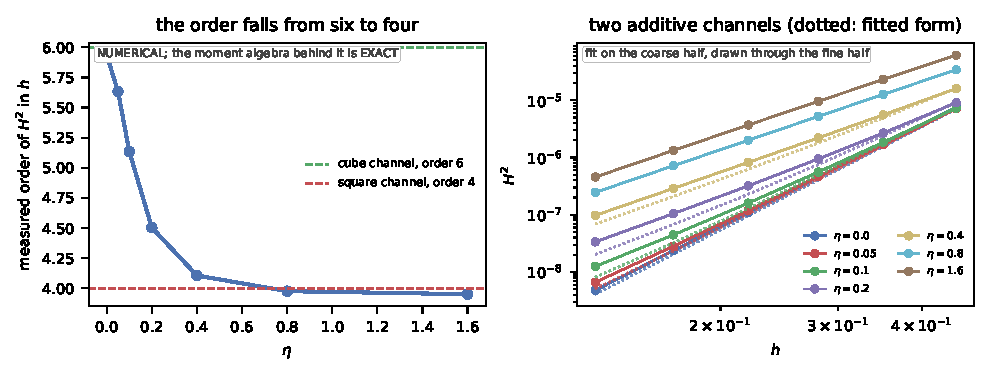
\includegraphics[width=\columnwidth]{paperB_crossover.pdf}
\caption{Left: the measured order in $h$ against $\eta$, falling from six to four. Right:
$H^{2}$ against $h$ at several $\eta$, with the two-channel form
$c_{6}h^{6}+c_{4}\eta^{2}h^{4}$ fitted on the coarse half and drawn through the fine half.
The crossover is at $\eta\asymp h$.}
\label{fig:crossover}
\end{figure}
\begin{figure}[t]
\centering
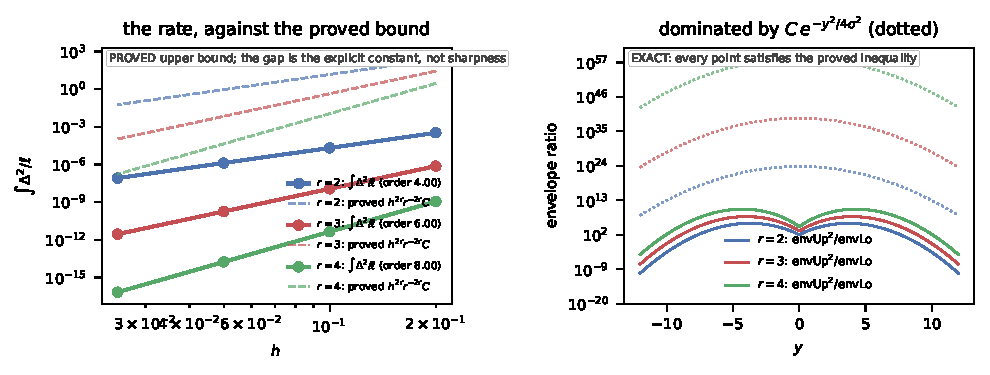
\includegraphics[width=\columnwidth]{paperB_envelope_rate.pdf}
\caption{The proved envelope chain. Left: $\int\Delta^{2}/\ell$ against $h$ for
$r=2,3,4$, with the measured orders $4.00$, $6.00$, $8.00$ and the proved bound
$h^{2r}r^{-2r}C$ dashed; the vertical gap is the explicit constant, which is not claimed
sharp. Right: the envelope ratio $\mathrm{envUp}^{2}/\mathrm{envLo}$ and the Gaussian
$C\,e^{-y^{2}/4\sigma^{2}}$ that dominates it, which is what makes the integral finite
without any polynomial-times-Gaussian integrability lemma.}
\label{fig:envrate}
\end{figure}
\begin{figure}[t]
\centering
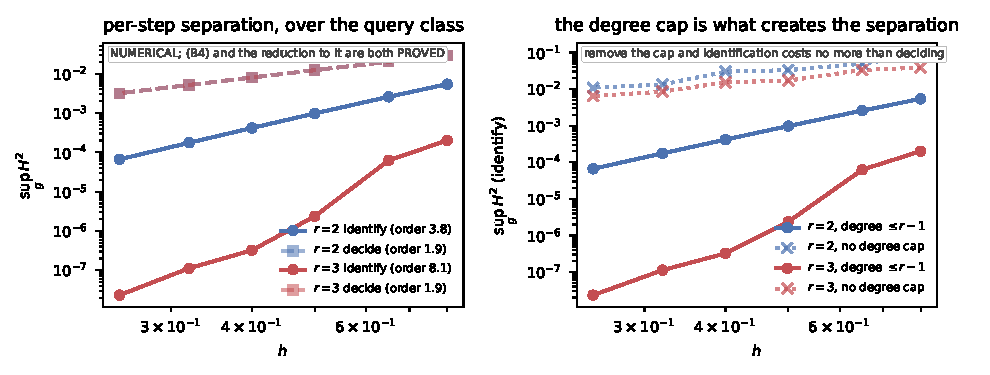
\includegraphics[width=\columnwidth]{paperB_uniform_hellinger.pdf}
\caption{Left: the per-step separation over the query class, for both directions. Right:
the same quantity with every class restriction removed --- the separation collapses, so
the restriction is what creates it. The degree-capped class is not shown: it is refuted in
the text by an exhibited probe, not by a search.}
\label{fig:unih}
\end{figure}

\begin{figure}[t]
\centering
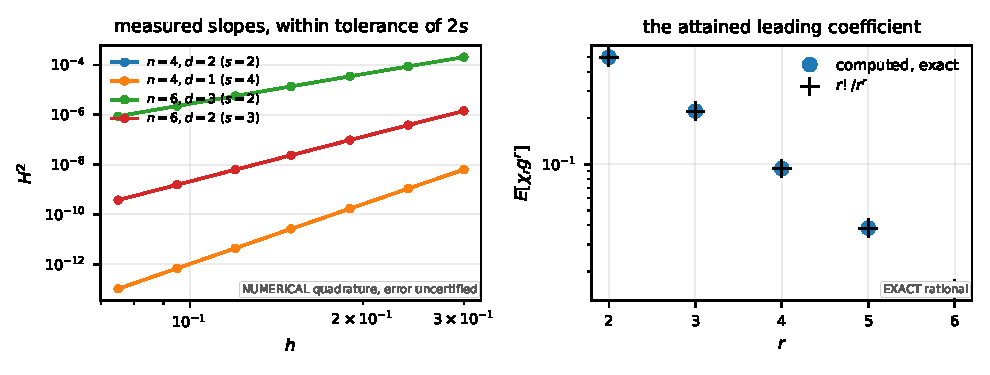
\includegraphics[width=\columnwidth]{paperB_orders.pdf}
\caption{Left: squared Hellinger against $h$. Right: the attained leading coefficient
against $r!/r^{r}$, in exact rational arithmetic.}
\label{fig:orders}
\end{figure}

\begin{figure}[t]
\centering
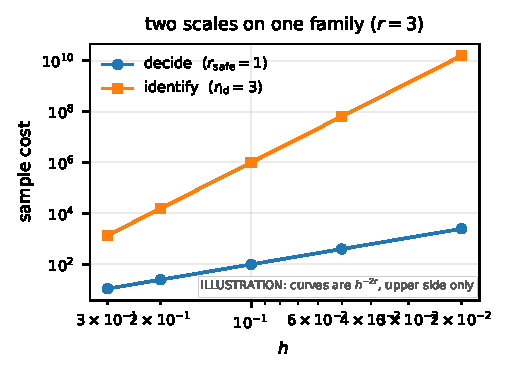
\includegraphics[width=0.78\columnwidth]{paperB_two_scales.pdf}
\caption{The two scales on one family. Marked as an illustration of the proved orders; the
empirical sample counts are reported separately.}
\label{fig:scales}
\end{figure}

\section{The two orders, on the real geometry, and a matching upper bound}
\label{sec:geometry}

The separation this paper is about is between two \emph{observation orders}: the order at
which a decision becomes safe, and the order at which the world becomes identified. Both
are defined on the real \lean{selectedRadius} geometry rather than on a stand-in.

Write $\theta\sim_{s}\lambda$ for indistinguishability at order $s$, and
$\mathrm{class}_{s}(\theta)$ for the class it induces. Two facts pin the orders.

\begin{theorem}[The two orders separate]
\label{thm:orders}
For $m\ge3$: every class at order $1$ has a common safe answer, no class at order $0$ does,
and identification holds at order $s$ if and only if $s\ge m-1$. Hence
$s_{\mathrm{safe}}=1$ while $s_{\mathrm{id}}=m-1$, and the gap grows with $m$.
\end{theorem}

The identification half is an \emph{iff}, so $m-1$ is tight on both sides rather than an
upper estimate. Two further facts say the geometry is the interesting one and not a
degenerate case: any two worlds share a safe answer at $m\ge3$
(\lean{safe\_sets\_overlap}), while no answer is safe for all of them
(\lean{no\_common\_safe\_all}). Overlapping-but-not-nested safe sets are exactly what makes
the safe order small and the identification order large. The order-$0$ class is an
obstruction (\lean{obstruction\_at\_order\_zero}), which is the hypothesis the
$\log(1/\delta)$ lower bound consumes, so the lower side is applied to a geometry that
verifiably satisfies it.

\leanbox{\lean{identifiableAt\_iff}, \lean{decidableAt\_of\_one\_le},
\lean{not\_decidableAt\_zero}, \lean{decide\_order\_lt\_identify\_order},
\lean{safe\_sets\_overlap}, \lean{no\_common\_safe\_all},
\lean{obstruction\_at\_order\_zero} in \lean{LeanPaperBGeometryV1}}

\NOTEPAR{What Theorem~\ref{thm:orders} is and is not. It is a statement about the
indistinguishability \emph{partition}: $\sim_{s}$ is defined directly on the world index,
as ``equal, or both at index at least $s$'', and the safe sets are the real
\lean{selectedRadius} ones. So the geometry is the model's, but the partition is posited
rather than \emph{derived} from what the queries can resolve. Turning
$s_{\mathrm{safe}}=1$ and $s_{\mathrm{id}}=m-1$ into a sample-complexity separation needs
one more step in each direction: $\sim_{s}$ must be shown to be exactly the relation
induced by the moments the query class can see up to order $s$, and then the lower bound
of Section~\ref{sec:adaptive} and the upper bound of Theorem~\ref{thm:lrt} apply to it.
Neither implication is proved here, and the two orders should not be quoted as sample
complexities until they are.}

\subsection{The upper bound, with its per-pair input derived}

An upper bound that \emph{assumes} a per-pair test bound assumes the result. Here the test
is exhibited and its error computed. Let $P,Q$ be the $N$-fold product laws of two
candidate worlds on a finite observation alphabet, and let the test declare the first world
exactly on the sequences it makes at least as likely. Its two error probabilities satisfy
\begin{equation}
\tfrac12\bigl(\mathrm{err}_{\mathrm{I}}+\mathrm{err}_{\mathrm{II}}\bigr)
=\tfrac12\sum_{t}\min\bigl(P(t),Q(t)\bigr),
\label{eq:lrtexact}
\end{equation}
an \emph{identity}, not a bound: the two sums recombine term by term. Bounding the minimum
by the geometric mean and tensorising the Hellinger affinity,
$\sum_{t}\sqrt{P(t)Q(t)}=\bigl(\sum_{o}\sqrt{p(o)q(o)}\bigr)^{N}=(1-H^{2})^{N}$, gives

\begin{theorem}[Per-pair test bound]
\label{thm:lrt}
If $H^{2}(p,q)\ge c$ then \emph{each} of the test's two error probabilities is at most
$\delta/K$ once $N\ge\log(K/\delta)/c$; over $K$ pairs each sums to at most $\delta$.
\end{theorem}

\begin{proof}
By \eqref{eq:lrtexact} the two errors sum to $\sum_{t}\min(P(t),Q(t))$. Since
$\min(a,b)^{2}\le ab$ for $a,b\ge0$, each summand is at most $\sqrt{P(t)Q(t)}$. Writing
$P(t)=\prod_{i}p(t_{i})$ and likewise for $Q$, the square root of the product is the
product of the square roots, and summing a product over all sequences factorises:
\[
\sum_{t}\sqrt{P(t)Q(t)}
=\sum_{t}\prod_{i}\sqrt{p(t_{i})q(t_{i})}
=\Bigl(\sum_{o}\sqrt{p(o)q(o)}\Bigr)^{N}
=(1-H^{2})^{N}.
\]
Now $1-x\le e^{-x}$ gives $(1-H^{2})^{N}\le e^{-NH^{2}}\le e^{-Nc}$, and
$N\ge\log(K/\delta)/c$ makes that at most $\delta/K$. Both error probabilities are
non-negative and their sum is bounded, so each is bounded separately --- which is the form
the union bound over the $K$ pairs consumes. Note the bound is on the sum, not on the
average: an earlier version halved it, which bounds neither world's own error.
\end{proof}

With $c=c_{0}h^{2r}$ this is $N=O\bigl(h^{-2r}\log(K/\delta)\bigr)$: the \emph{same}
exponent in $h$ that the lower bound produces, so the two sides match in order. The
$\delta$-dependence matches only up to a constant, which \lean{bounds\_same\_order} makes
explicit. The separation $c_{0}h^{2r}\le H^{2}$ is an input to this theorem --- it is what
Section~\ref{sec:law} supplies on the linear class --- and the two are not yet composed
into a single statement; \lean{separation\_nonvacuous} exhibits laws with $0<H^{2}<1$ so
the theorem is not vacuous.

\leanbox{\lean{affinity\_prodLaw}, \lean{err\_eq\_sum\_min},
\lean{err\_le\_affinity\_pow}, \lean{lrt\_error\_le},
\lean{identify\_sample\_complexity}, \lean{decoder\_total\_error},
\lean{separation\_nonvacuous} in \lean{LeanPaperBTestV1}; \lean{decoder\_union\_bound},
\lean{bounds\_same\_order} in \lean{LeanPaperBGeometryV1}}

\subsection{The crossover: the mechanism, not a sweep}
\label{sec:crossover}

Widening the probe to $g_{\eta}=(z_{4}+z_{5}+z_{6}+\eta z_{4}z_{5})/(3+\eta)$ is expected
to give $H^{2}\asymp h^{6}+\eta^{2}h^{4}$. A sweep of fitted slopes cannot decide that
shape, because it cannot see whether the two scales \emph{add} or \emph{interfere}: that
turns on a cross term. The algebra settles it.

Against the hidden character $\chi=z_{4}z_{5}z_{6}$,
\[
\mathbb{E}[\chi g_{\eta}]=0,\qquad
\mathbb{E}[\chi g_{\eta}^{2}]=\frac{2\eta}{(3+\eta)^{2}},\qquad
\mathbb{E}[\chi g_{\eta}^{3}]=\frac{6}{(3+\eta)^{3}},
\]
all three exact. The density difference between $v=+1$ and $v=-1$ then expands with an odd
channel $A(y)=f''(y-1)-f''(y+1)$ at coefficient $\eta h^{2}/(3+\eta)^{2}$ and an even
channel $B(y)=f'''(y-1)-f'''(y+1)$ at coefficient $h^{3}/(3+\eta)^{3}$.

\begin{theorem}[The cross term vanishes by parity]
\label{thm:parity}
If $A$ is odd, $B$ is even and the base density $p_{0}$ is even, then $AB/p_{0}$ is odd and
$\int AB/p_{0}=0$. Consequently
$\int(\alpha A+\beta B)^{2}/p_{0}=\alpha^{2}\int A^{2}/p_{0}+\beta^{2}\int B^{2}/p_{0}$,
and substituting the two coefficients gives exactly $\eta^{2}h^{4}$ plus $h^{6}$.
\end{theorem}

Numerically, on the model's own baseline --- the mixture $p_{0}(y)=\tfrac12[f(y-1)+f(y+1)]$
over the $z_{1}$ channel, not the head density $f$ alone, which an earlier version of the
check used --- the normalised cross term is $6.6\times10^{-15}$.

\NOTEPAR{Three things stand between this mechanism and the law, and none is proved: that
$A$ and $B$ are not identically zero, that the two integrals are finite, and that the
remainder is bounded \emph{uniformly in} $(h,\eta)$. It is also a law for the single probe
$g_{\eta}$; a class-level crossover needs the widened class defined and a uniform upper
bound over it. The measured orders $5.93\to3.95$ are evidence, not proof.}

\leanbox{\lean{moment\_one}, \lean{moment\_two}, \lean{moment\_three},
\lean{integral\_odd\_eq\_zero}, \lean{cross\_term\_vanishes},
\lean{quadratic\_splits}, \lean{two\_scale\_shape}, \lean{crossover\_balance} in
\lean{LeanPaperBCrossoverV1}}

\section{Limitations}
\label{sec:limits}

\begin{enumerate}
\item[1)] \textbf{The general rate is not proved.} Matching orders are established on
one family; Theorem~\ref{thm:classes} and Theorem~\ref{thm:floor} are the combinatorial half
of the general law, not the law.
\item[2)] \textbf{The transcript results are discrete.} Theorem~\ref{thm:chain} is proved
for a finite observation alphabet, a deterministic policy and a fixed horizon. On the
Gaussian model we do not run that argument at all; we run the affinity route of
\eqref{eq:affinity}, whose arithmetic is proved and whose analytic input---a per-step
Hellinger bound uniform over $g$, with an integrable envelope---is now proved as well
(\lean{hellinger\_rate\_bound}). What remains open at this point is only the passage from a
single step to an adaptive randomised transcript. Replacing $N$
by $\mathbb{E}\tau$ needs a stopped-transcript identity and must not be done by substitution.
\item[3)] \textbf{Constants depend on $r$.} Nothing here is uniform as $r$ grows with a
budget.
\item[4')] \textbf{The estimator's error is now a statement about the measure.} Chebyshev
is proved for a real random variable, the cross terms of the empirical sum vanish by
independence and centring, and the two combine into
$\Pr(|\sum_{i}Z_{i}|\ge Nt)\le V/Nt^{2}$ --- the bound the sample budgets consume, about the
measure of an event rather than a rearrangement. What is still cited is nothing: at fixed
error, Chebyshev suffices and no exponential tail is needed.
\leanbox{\lean{chebyshev\_real}, \lean{cross\_term\_zero}, \lean{second\_moment\_sum},
\lean{estimator\_error\_le} in \lean{LeanPaperBRatesV1}}
\item[4)] \textbf{Upper bounds: the per-pair input is now derived, on a finite
alphabet.} Theorem~\ref{thm:lrt} replaces the assumed per-pair error level with the error
of an exhibited test, computed exactly by \eqref{eq:lrtexact} and bounded by affinity
tensorisation. It is proved for a \emph{finite} observation alphabet; the Gaussian model of
\eqref{eq:obs} is not covered by it, and carrying it across is the same analytic step as
item 2). What follows is the older statement about the variance input, which remains.
\textbf{Variance input.} The variance input the Chebyshev
budget needs is now proved for the \emph{observation} and not only for the cube: the signal
$F+hg$ is bounded by a constant independent of $h$, so every absolute moment of $Y$ is at
most $2^{n}(B_{0}^{n}+G_{n})$ with $G_{n}$ the noise's own $n$-th moment, finite because all
moments of a Gaussian are. The cube bound $9^{4}$ could not be carried across --- Gaussian
noise has unbounded support, so no bound on $|Y|$ exists at all. What is still cited rather
than proved is the estimator's concentration itself.
\item[5)] \textbf{Finitely many worlds and queries} throughout Section~\ref{sec:law}.
\end{enumerate}

\section{Conclusion}

On one family the cost of choosing a safe compression and the cost of identifying the world
separate by a computable order, and the separation is supported from both sides: the moment
law is proved to vanish below the order and to be attained at it with an exact constant, and
the lower bound is proved against every adaptive policy on a finite observation alphabet by
building the transcript law from the policy, and on the Gaussian model is reduced, with the
reduction proved, to a single per-step Hellinger bound uniform over the query class. The
general law's combinatorial half---which groupings suffice, and why a surviving obstruction
is costly even for randomised rules---is proved; the analytic half, which would turn an
order into a rate for an arbitrary family, is not, and we have said so where the claim would
otherwise be made.

\section*{Companion material}
Two files accompany this paper and are part of the submission record.
\texttt{PROOFS.md} gives the central arguments as readable mathematics with no Lean
required --- setup, claim, proof, and in the same breath what the claim does not
cover. \texttt{DOSSIER.md} carries the full state: every audited theorem, every
measured number with its artifact and provenance status, the open list, and the
claims retracted during preparation, recorded rather than silently edited.
\texttt{CLAIMS.md} is the one-row-per-headline table of claim, final theorem,
remaining hypotheses and evidence.

\begin{thebibliography}{00}

\bibitem{duc2015} A. Duc, S. Faust, and F.-X. Standaert, ``Making masking security
proofs concrete,'' IACR ePrint 2015/119, 2015.

\bibitem{poli2023} M. Poli et al., ``Ideal abstractions for decision-focused learning,''
arXiv:2303.17062, 2023.


\bibitem{javdani2014} S. Javdani, Y. Chen, A. Karbasi, A. Krause, D. Bagnell, and
S. Srinivasa, ``Near optimal Bayesian active learning for decision making,'' in
\emph{Proc. 17th Int. Conf. Artificial Intelligence and Statistics (AISTATS)}, 2014,
pp.~430--438.

\bibitem{grosso2014} V. Grosso, F.-X. Standaert, and E. Prouff, ``Low entropy masking
schemes, revisited,'' in \emph{Smart Card Research and Advanced Applications (CARDIS)},
2013, pp.~33--43.

\bibitem{rioul2021} O. Rioul, W. Cheng, and S. Guilley, ``Cumulant expansion of mutual
information for quantifying leakage of a protected secret,'' in \emph{Proc. IEEE Int. Symp.
Information Theory (ISIT)}, 2021, pp.~2596--2601.

\bibitem{degenne2019} R. Degenne and W. M. Koolen, ``Pure exploration with multiple correct
answers,'' in \emph{Advances in Neural Information Processing Systems 32}, 2019,
pp.~14591--14600.

\bibitem{wangyou2026} Z. Wang and K. You, ``Information games with multiple correct answers
and piecewise-convex alternative sets,'' arXiv:2606.21889, 2026.

\bibitem{odonnell2014} R. O'Donnell, \emph{Analysis of Boolean Functions}. Cambridge,
U.K.: Cambridge Univ. Press, 2014.

\bibitem{tsybakov2009} A. B. Tsybakov, \emph{Introduction to Nonparametric Estimation}.
New York, NY: Springer, 2009.

\bibitem{mathlib2020} The mathlib Community, ``The Lean mathematical library,'' in
\emph{Proc. 9th ACM SIGPLAN Int. Conf. Certified Programs and Proofs (CPP)}, 2020,
pp.~367--381.

\bibitem{demoura2021} L. de Moura and S. Ullrich, ``The Lean 4 theorem prover and
programming language,'' in \emph{Proc. 28th Int. Conf. Automated Deduction (CADE)}, 2021,
pp.~625--635.

\end{thebibliography}

\end{document}
